\documentclass[11pt,a4paper]{article}
\usepackage[utf8]{inputenc}\usepackage[T1]{fontenc}
\usepackage[margin=1in]{geometry}
\usepackage{amsmath,amssymb,booktabs,graphicx,enumitem,xcolor,parskip,titlesec}
\usepackage[hidelinks]{hyperref}
\graphicspath{{figures/}}
\definecolor{qnavy}{RGB}{20,40,75}\definecolor{qgrey}{RGB}{90,90,90}\definecolor{qred}{RGB}{150,30,30}
\titleformat{\section}{\large\bfseries\color{qnavy}}{\thesection}{0.6em}{}
\begin{document}\thispagestyle{empty}
\noindent
{\large\bfseries\color{qnavy} Report R06 --- Chromatin-Regulator Mutations and Survival in NSCLC}\\[2pt]
{\color{qgrey}The reframed lung arm. One cohort, not two --- the audit withdrew the replication claim.}\\[6pt]
{\color{qgrey}\rule{\textwidth}{0.4pt}}

\medskip
\noindent 7 August 2026 \quad\textbullet\quad Quantara

\section*{Summary}

The response letter proposed abandoning the acquired-resistance framing, which public data
cannot power, in favour of chromatin dysregulation. This report tests that directly on
mutation and survival data --- no imaging, no methylation download required.

In the MSK NSCLC circulating-tumour-DNA cohort (\textbf{$n=1{,}127$, 618 events}),
\textbf{KEAP1} (HR 2.07, 95\% CI 1.63--2.62, $q<0.0001$) and \textbf{SMARCA4} (HR 1.73,
1.27--2.35, $q=0.0009$) mutations are both associated with shorter overall survival. Median
survival falls from 28.8 to 11.3 months with KEAP1 mutation and from 28.4 to 18.2 months with
SMARCA4. Both pre-registered positive controls were recovered at expected magnitudes
(STK11 HR 1.63, $q=0.0004$; TP53 HR 1.25, $q=0.0074$).

\textbf{This is a single-cohort finding.} The run's decision line claimed SMARCA4 replicated
across two cohorts; the audit withdrew that, for reasons in \S3.

\section{Results --- MSK NSCLC ctDx cohort ($n=1{,}127$)}

\begin{center}
\begin{tabular}{@{}lrrccr@{}}
\toprule
\textbf{Gene} & \textbf{Mutated} & \textbf{HR} & \textbf{95\% CI} & \textbf{$q$ (BH)} &
\textbf{Median OS, mut vs WT} \\
\midrule
\textbf{KEAP1} & 113 & \textbf{2.07} & 1.63--2.62 & $<0.0001$ & 11.3 vs 28.8 mo \\
\textbf{SMARCA4} & 57 & \textbf{1.73} & 1.27--2.35 & 0.0009 & 18.2 vs 28.4 mo \\
KMT2D & 39 & 0.98 & 0.65--1.49 & 0.94 & 27.8 vs 27.4 mo \\
\midrule
STK11 \emph{(control)} & 106 & 1.63 & 1.27--2.10 & 0.0004 & 14.0 vs 28.0 mo \\
TP53 \emph{(control)} & 580 & 1.25 & 1.07--1.46 & 0.0074 & 23.8 vs 32.3 mo \\
\bottomrule
\end{tabular}
\end{center}

\begin{center}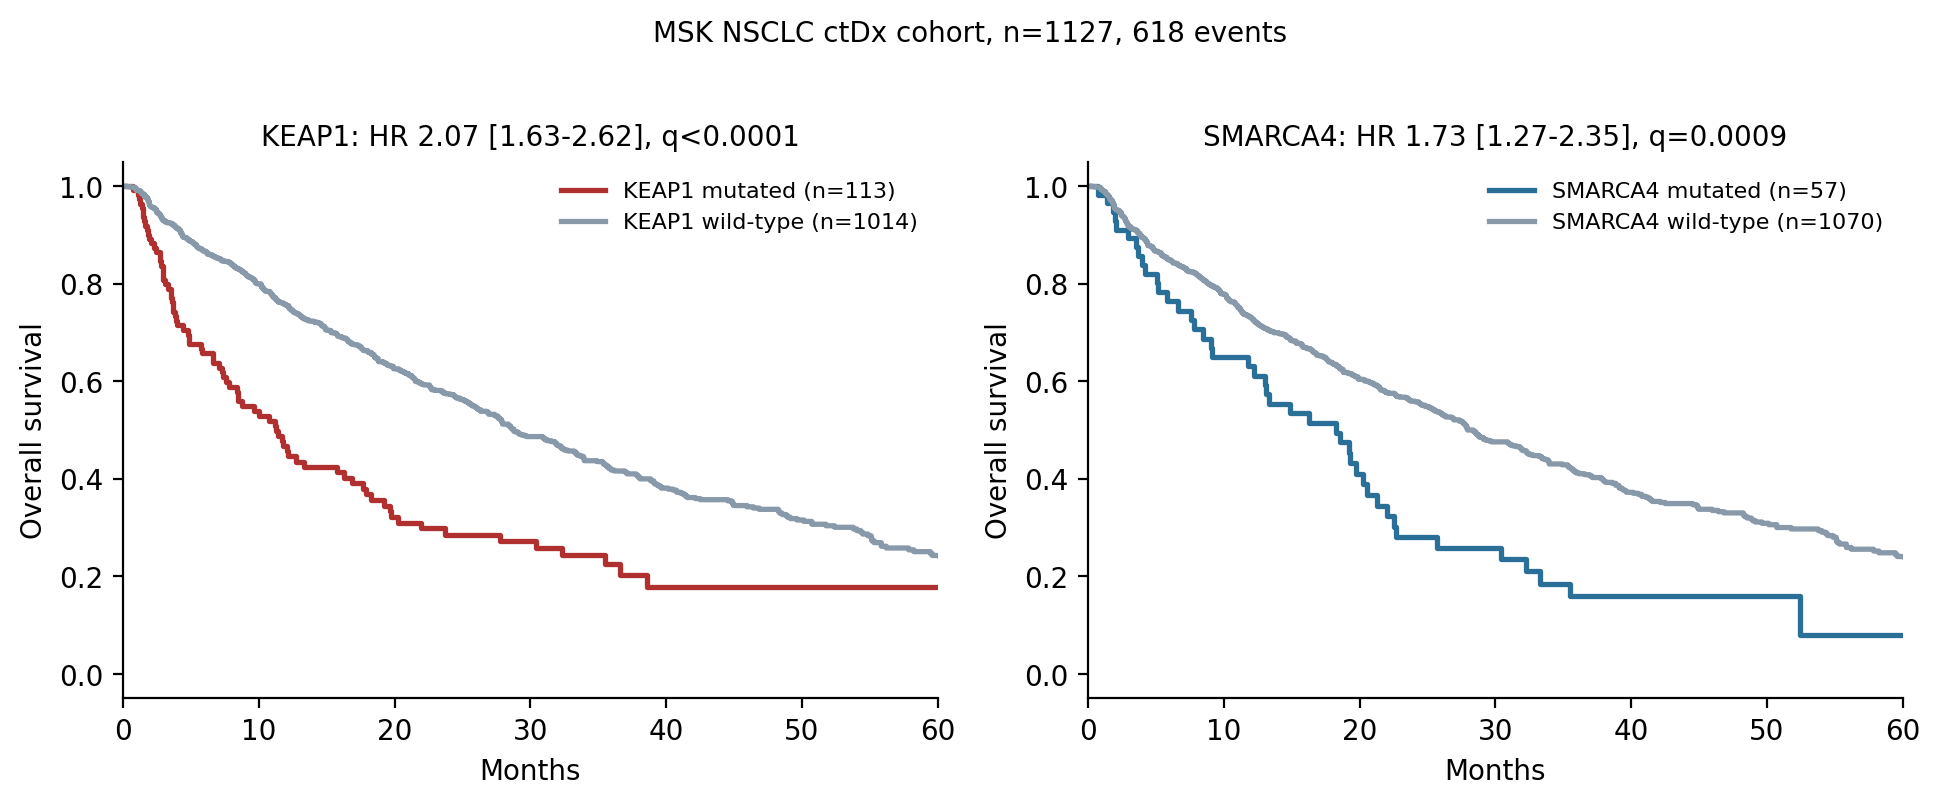
\includegraphics[width=\textwidth]{fig1_km_keap1_smarca4.png}\end{center}

\section{\textcolor{qred}{Why the replication claim was withdrawn}}

The second cohort (\texttt{luad\_mskcc\_2020}, $n=604$) appeared to corroborate SMARCA4 at
HR 3.97 ($q=0.001$). It cannot be used for that purpose:

\begin{itemize}[leftmargin=1.4em,nosep]
\item It has only \textbf{45 events among 604 patients (7\%)}.
\item \textbf{It fails its own positive controls.} TP53 HR 1.18 ($p=0.58$) and STK11 HR 1.04
($p=0.91$) --- two established NSCLC prognostic factors, both undetected. A cohort that
cannot find STK11 or TP53 cannot corroborate SMARCA4.
\item Its SMARCA4 estimate rests on \textbf{9 events among 33 mutants}, with a confidence
interval spanning 1.90--8.29.
\item KEAP1 pointed in \emph{opposite} directions between the two cohorts (HR 0.87 vs 2.07),
which is the signature of an underpowered comparison.
\item \textbf{KMT2D's reported HR of 0.000 is a degenerate fit, not an estimate} --- there
are zero events among its 28 mutants, so the hazard ratio is not estimable. It should not
have been printed as a number.
\end{itemize}

\noindent
The honest statement is therefore single-cohort, well-controlled, and not yet replicated.

\section{Interpretation}

KEAP1 and SMARCA4 both plausibly belong to the same biology the reframed arm targets. KEAP1
loss deregulates the NRF2 oxidative-stress programme; SMARCA4 is a core SWI/SNF chromatin
remodeller. That SMARCA4 is prognostic here is consistent with the SWI/SNF
tyrosine-kinase-inhibitor-resistance literature that motivated the original lung manuscript
--- but as a prognostic association in a mostly treatment-heterogeneous cohort, not as
evidence of a resistance mechanism.

KMT2D, the third chromatin regulator and the one with the largest patient count in our
earlier inventory, is \textbf{null} (HR 0.98). The reframed arm should not be built on KMT2D.

\section{Limitations}

\begin{itemize}[leftmargin=1.4em,nosep]
\item \textbf{Single cohort.} Replication requires a second adequately powered cohort;
neither of ours qualifies.
\item \textbf{Targeted panel, circulating tumour DNA.} Mutation detection depends on tumour
shedding, and ctDNA-positive disease is itself prognostically adverse. Effect sizes may
partly reflect detectability.
\item \textbf{No treatment adjustment.} The cohort spans heterogeneous therapy; no line of
treatment or regimen was adjusted for.
\item \textbf{No methylation.} The chromatin-\emph{dysregulation} framing would be far
stronger with the methylome. That download (TCGA-LUAD/LUSC, 1{,}283 open files) remains the
main funded extension.
\item Repository \texttt{data\_mutations.txt} for both cohorts are 132-byte git-LFS pointer
stubs whose objects are unretrievable upstream; all mutation data here came from the
cBioPortal REST API instead. Recorded as gate G1.
\end{itemize}

\section{Audit}

\begin{center}
\begin{tabular}{@{}llp{7.0cm}@{}}
\toprule
\textbf{Check} & \textbf{Verdict} & \textbf{Finding} \\
\midrule
Positive controls, large cohort & \textbf{Both recovered} & STK11 $q=0.0004$; TP53 $q=0.0074$ \\
Positive controls, small cohort & \textbf{Both FAILED} & TP53 $p=0.58$; STK11 $p=0.91$ --- cohort unusable for corroboration \\
Event adequacy & \textbf{Small cohort inadequate} & 45 events / 604 patients; SMARCA4 rests on 9 events \\
Degenerate fits & \textbf{One found} & KMT2D HR 0.000, zero events among 28 mutants; not estimable \\
Direction consistency & \textbf{KEAP1 inconsistent} & HR 0.87 vs 2.07 across cohorts \\
Gates & \textbf{7 / 7 PASS} & Patient counts, API retrieval, survival counts, controls \\
\bottomrule
\end{tabular}
\end{center}

\noindent
\textbf{Note on the evidence bundle:} \texttt{results.json} contains a
\texttt{\_decision} field stating that SMARCA4 replicates. That line reflects the
pre-specified rule as mechanically applied and is \emph{superseded by this report}. The
decision fields in run artefacts should not be cited without the accompanying audit.

\section{How to verify}

\texttt{evidence/results.json} holds every hazard ratio, confidence interval and $q$-value
for both cohorts. \texttt{config.yaml} (hash \texttt{d3919b85\ldots}) was written before any
outcome was read. Mutation retrieval is reproducible with the API call in
\texttt{m6\_lung\_chromatin.py}.

\vfill
\noindent{\color{qgrey}\rule{\textwidth}{0.4pt}}\\
{\footnotesize\color{qgrey}Run \texttt{runs/20260807T081212Z-R06lungchrom-3f8bece}. Data:
cBioPortal \texttt{nsclc\_ctdx\_msk\_2022} and \texttt{luad\_mskcc\_2020}, ODbL. No
patient-level identifiers reproduced.}
\end{document}
